\documentclass[11pt]{article}

\usepackage[margin=1in]{geometry}
\usepackage{booktabs}
\usepackage{array}
\usepackage{longtable}
\usepackage{hyperref}
\usepackage{xcolor}
\usepackage{tikz}
\usepackage{amsmath}
\usepackage{fancyhdr}
\usepackage{caption}
\usetikzlibrary{arrows.meta,positioning,shapes.geometric,fit,calc}

\hypersetup{
  colorlinks=true,
  linkcolor=blue!60!black,
  urlcolor=blue!60!black,
  citecolor=blue!60!black
}

\pagestyle{fancy}
\setlength{\headheight}{14pt}
\fancyhf{}
\lhead{DLR-Lambda Worklist Experiment}
\rhead{Nikit Phadke}
\cfoot{\thepage}

\newcommand{\code}[1]{\texttt{\detokenize{#1}}}
\newcommand{\pass}{\textsc{pass}}
\newcommand{\fail}{\textsc{fail}}
\newcolumntype{L}[1]{>{\raggedright\arraybackslash}p{#1}}
\setlength{\emergencystretch}{2em}

\title{\textbf{From Batch Reduction to Investigative Fixpoint:}\\
A DLR-Lambda-2 Experiment on Marker-Free Log Diagnosis}
\author{Nikit Phadke}
\date{June 2026}

\begin{document}
\maketitle

\begin{abstract}
The first DLR-lambda Loghub experiment showed that typed recursive control can
compose distributed log evidence into a ProcessIR causal diagnosis. Its control
plan, however, was still batch-shaped: split, map, filter, reduce, output. This
paper freezes the next finding. Some incidents are not merely distributed; their
later evidence changes the meaning of earlier evidence. In such cases, event
recall is not enough. The controller must treat certain facts as frontier items,
schedule follow-up retrieval, reconcile contradictions, revise hypotheses, and
iterate until the ProcessIR reaches a verified fixpoint. We implement a
marker-free Loghub experiment comparing one-pass MapReduce-style DLR-lambda
against a typed worklist/fixpoint controller. Both systems recover all observed
event nodes. The MapReduce system still fails: it misses the expired-exemption
latent condition, mishandles contradiction, fails hypothesis revision, and does
not detect the local approval as a false terminal state. The worklist/fixpoint
system recovers all event nodes, latent conditions, causal edges, root causes,
and terminal-state diagnostics. The result supports a spectrum view:
MapReduce-style DLR-lambda is sufficient when evidence is independent and
reduction is associative; worklist/fixpoint DLR-lambda is needed when facts
generate follow-up obligations and later evidence revises earlier meaning.
\end{abstract}

\section{Introduction}

Operational diagnosis is often described as a search over evidence. That is only
partly true. In harder incidents, a fact is not merely an observation to store.
It is an obligation to investigate. A local service reports success, but the
parent workflow may still be invalid. A cached policy is used, but its freshness
must be checked. An exemption is claimed, but its validity at transition time
must be verified. An authority is asserted, but its domain must be confirmed.

The first DLR-lambda experiment \cite{dlr_lambda_1} used a simple
lambda-style recursive plan over Loghub Linux logs: split the trace into
chunks, map chunks to event frames, filter incident evidence, and reduce the
frames into ProcessIR. That experiment established a useful lower rung: when
evidence is separated but mostly independent, batch-style recursive composition
can recover a latent stale-representation root cause.

This paper asks a sharper question:

\begin{quote}
What happens when a later fact changes the meaning of an earlier fact?
\end{quote}

The answer is that MapReduce is no longer the right conceptual center. It is a
special case. DLR-lambda-2 is better modeled as typed recursive control over an
evidence graph until the relevant motif obligations reach fixpoint. In this
paper we implement the intermediate form, a worklist/fixpoint controller. We do
not yet make motif obligations a first-class calculus. Instead, we show why the
worklist layer is necessary and where the next semantic layer should attach.

\section{The Spectrum}

DLR-lambda should not be presented as a single execution plan. Different
diagnostic problems need different control strength. Table
\ref{tab:spectrum} summarizes the emerging spectrum.

\begin{table}[h]
\centering
\caption{A spectrum of DLR-lambda control.}
\label{tab:spectrum}
\small
\begin{tabular}{L{0.18\linewidth}L{0.30\linewidth}L{0.42\linewidth}}
\toprule
Stage & Center & Appropriate when \\
\midrule
DLR-lambda-1 & MapReduce composition & Evidence is distributed, mostly independent, and reduction is close to associative. \\
DLR-lambda-2 & Worklist/fixpoint investigation & Facts can change the meaning of prior facts and require scheduled follow-up joins. \\
DLR-lambda-3 & Motif obligation calculus & The system must prove that mandatory structural obligations are satisfied, violated, or explicitly unknown. \\
\bottomrule
\end{tabular}
\end{table}

This is not a replacement story. Many users will only need DLR-lambda-1. A log
classification pipeline, document triage system, or retrieval job may only need
bounded extraction plus final composition. DLR-lambda-2 is needed when evidence
creates unresolved frontier items. DLR-lambda-3 becomes necessary when terminal
validity itself must be formalized as an obligation-discharge problem.

\section{Background}

\subsection{DLR ProcessIR}

Disentangled Language Representation (DLR) represents traces as typed process
diagnoses rather than unstructured summaries. The relevant ProcessIR fields are
event frames, latent conditions, typed causal edges, root causes, false terminal
states, violated invariants, hypothesis revisions, prescriptions, and
confidence. This paper focuses on a specific ProcessIR failure pattern: a local
transition reports success while the parent process has not reached a valid
terminal state.

\subsection{Lambda-Style Control}

Lambda-RLM argues that long-context reasoning can be made more reliable by
expressing recursive control with typed functional primitives rather than
unbounded code generation or a single monolithic prompt \cite{lambda_rlm}. The
DLR-lambda experiments borrow this control idea but use ProcessIR as the target
representation. Recursive control answers how evidence is traversed. ProcessIR
answers what semantic object is recovered.

\subsection{MapReduce as a Special Case}

The DLR-lambda-1 control plan was:

\begin{verbatim}
SPLIT -> MAP -> FILTER -> REDUCE -> OUTPUT
\end{verbatim}

This is useful but structurally limited. It assumes that chunks can be processed
mostly independently, that extraction can precede global context, that one
reduction pass is enough, and that evidence relevance is known early. Those
assumptions break when an extracted fact creates a new question that must be
answered before the diagnosis can terminate.

\section{DLR-Lambda-2}

The DLR-lambda-2 control plan is:

\begin{verbatim}
INGEST -> EXTRACT -> JOIN -> SCHEDULE FOLLOW-UP
       -> RECONCILE -> FIXPOINT -> VERIFY -> ProcessIR
\end{verbatim}

The key difference is that the controller maintains typed evidence state. It can
derive hypotheses, schedule new work, weaken or retract prior hypotheses, and
stop only when the graph reaches a coverage-checked fixpoint.

\begin{figure}[h]
\centering
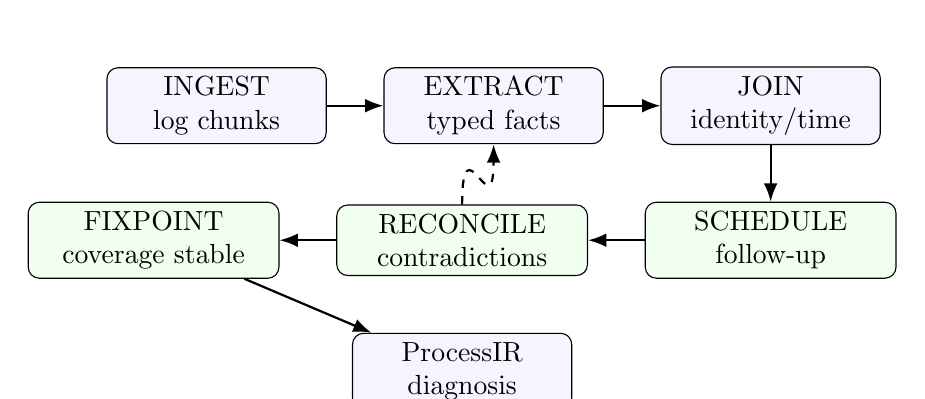
\begin{tikzpicture}[
  node distance=0.72cm,
  box/.style={draw, rounded corners, align=center, minimum height=0.75cm,
    text width=2.55cm, fill=blue!4},
  strong/.style={draw, rounded corners, align=center, minimum height=0.75cm,
    text width=2.95cm, fill=green!6},
  arr/.style={-Latex, thick}
]
\node[box] (ingest) {INGEST\\log chunks};
\node[box, right=of ingest] (extract) {EXTRACT\\typed facts};
\node[box, right=of extract] (join) {JOIN\\identity/time};
\node[strong, below=of join] (schedule) {SCHEDULE\\follow-up};
\node[strong, left=of schedule] (reconcile) {RECONCILE\\contradictions};
\node[strong, left=of reconcile] (fixpoint) {FIXPOINT\\coverage stable};
\node[box, below=of reconcile] (out) {ProcessIR\\diagnosis};
\draw[arr] (ingest) -- (extract);
\draw[arr] (extract) -- (join);
\draw[arr] (join) -- (schedule);
\draw[arr] (schedule) -- (reconcile);
\draw[arr] (reconcile) -- (fixpoint);
\draw[arr] (fixpoint) -- (out);
\draw[arr, dashed] (reconcile.north) .. controls +(0,1.1) and +(0,-1.1) .. (extract.south);
\end{tikzpicture}
\caption{DLR-lambda-2 as typed investigative fixpoint. Reconciliation can
schedule more extraction before the ProcessIR is terminal-valid.}
\end{figure}

\section{Experimental Design}

\subsection{Dataset}

The experiment uses the public Loghub Linux sample as a noisy carrier
\cite{loghub_repo,loghub_issre,loghub2_issta}. The original Linux log lines are
left intact. Seven marker-free synthetic lines are injected into the trace,
producing 2007 total lines. Unlike the first DLR-lambda experiment, the
injected evidence does not use an explicit \code{DLR_LAMBDA} marker. The parser
must recover the incident using ordinary textual evidence such as refund IDs,
policy versions, exemption identifiers, audit observations, and settlement
outcomes.

\subsection{Incident}

The incident is designed around a meaning-changing later fact. A refund is
approved using policy version v17 after policy version v18 exists. However, the
approval claims VIP exemption \code{EX-77}, which could make the apparent
policy mismatch valid. The exemption therefore weakens the stale-policy
hypothesis and creates a follow-up obligation: was \code{EX-77} valid at the
time of approval? A later line reveals that the exemption expired before
approval. The final diagnosis must therefore revise the hypothesis and treat the
local approval as a false terminal state.

\begin{table}[h]
\centering
\caption{Distributed marker-free evidence.}
\label{tab:evidence}
\small
\begin{tabular}{r p{0.76\linewidth}}
\toprule
Line & Evidence summary \\
\midrule
117 & Local policy cache has TTL 1800s and requires current policy before terminal approval. \\
444 & Refund policy changes to version v18, requiring manager review unless an active VIP exemption exists. \\
809 & Worker approves refund R-914 using policy v17 and claims exemption EX-77. \\
1044 & Entitlements service asserts VIP exemption EX-77 for the refund. \\
1377 & Entitlements service states that EX-77 expired before approval. \\
1600 & Audit observes v18 expected, v17 observed, and manager review missing. \\
1817 & Finance blocks settlement because approval was not terminal-valid. \\
\bottomrule
\end{tabular}
\end{table}

\subsection{Systems Compared}

The benchmark compares two systems:

\begin{enumerate}
  \item \textbf{One-pass MapReduce DLR-lambda}: scans chunks once, extracts
  primary facts, and performs a single reduction into ProcessIR. It does not
  schedule follow-up retrieval for exemption validity.
  \item \textbf{Worklist/fixpoint DLR-lambda}: scans chunks, stores typed
  facts, treats exemption and terminal claims as frontier items, schedules
  follow-up searches, revises hypotheses, verifies terminal evidence, and emits
  ProcessIR after fixpoint.
\end{enumerate}

\section{Gold Diagnosis}

The gold root causes are:

\begin{itemize}
  \item \code{lc_stale_policy_representation}: local approval used policy v17
  after authoritative policy v18 existed;
  \item \code{lc_expired_vip_exemption}: the apparent exemption existed but
  expired before approval.
\end{itemize}

The false terminal state is the local approval. It is locally successful, but
globally invalid because the policy version is stale, the exemption is expired,
the manager-review invariant is missing, and downstream settlement is blocked.

\begin{figure}[h]
\centering
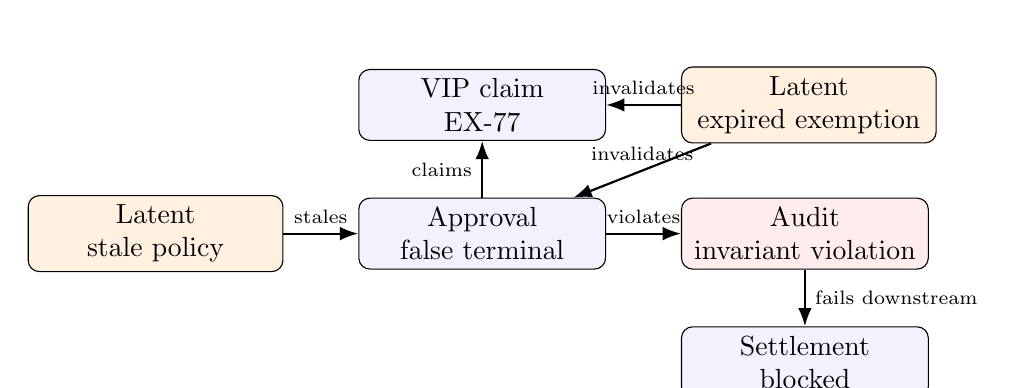
\begin{tikzpicture}[
  node distance=0.72cm and 0.95cm,
  latent/.style={draw, rounded corners, align=center, fill=orange!12,
    text width=3.0cm, minimum height=0.84cm},
  event/.style={draw, rounded corners, align=center, fill=blue!5,
    text width=2.9cm, minimum height=0.84cm},
  bad/.style={draw, rounded corners, align=center, fill=red!7,
    text width=2.9cm, minimum height=0.84cm},
  arr/.style={-Latex, thick}
]
\node[latent] (stale) {Latent\\stale policy};
\node[event, right=of stale] (approval) {Approval\\false terminal};
\node[event, above=of approval] (claim) {VIP claim\\EX-77};
\node[latent, right=of claim] (expired) {Latent\\expired exemption};
\node[bad, right=of approval] (audit) {Audit\\invariant violation};
\node[event, below=of audit] (settle) {Settlement\\blocked};
\draw[arr] (stale) -- node[above, font=\scriptsize]{stales} (approval);
\draw[arr] (approval) -- node[left, font=\scriptsize]{claims} (claim);
\draw[arr] (expired) -- node[above, font=\scriptsize]{invalidates} (claim);
\draw[arr] (expired) -- node[above, font=\scriptsize]{invalidates} (approval);
\draw[arr] (approval) -- node[above, font=\scriptsize]{violates} (audit);
\draw[arr] (audit) -- node[right, font=\scriptsize]{fails downstream} (settle);
\end{tikzpicture}
\caption{Gold diagnosis. The exemption claim is not an answer; it is a frontier
item whose validity must be joined against time and authority evidence.}
\end{figure}

\section{Results}

\begin{table}[h]
\centering
\caption{System-level scores.}
\label{tab:scores}
\scriptsize
\begin{tabular}{L{0.29\linewidth}rrrrrcccc}
\toprule
System & Conf. & Event & Latent & Edge & Root & Contr. & Rev. & Cov. & False \\
 & & recall & recall & recall & cause & & & & terminal \\
\midrule
One-pass MapReduce DLR-lambda & 0.62 & 1.00 & 0.50 & 0.83 & 0.50 & no & no & 0.67 & no \\
Worklist/fixpoint DLR-lambda & 0.88 & 1.00 & 1.00 & 1.00 & 1.00 & yes & yes & 1.00 & yes \\
\bottomrule
\end{tabular}
\end{table}

The crucial result is that the one-pass MapReduce system achieves perfect event
node recall and still fails. It sees the primary events, including the approval,
VIP exemption claim, audit violation, and settlement block. It misses the
expired-exemption latent condition because it does not compile the exemption
claim into a scheduled follow-up search. As a result, it also misses the
hypothesis revision and fails to mark the approval as a false terminal state.

The worklist/fixpoint system passes all reported criteria. It treats the
approval's exemption as unresolved, schedules \code{follow_exemption_EX-77},
finds the expiration evidence, revises the hypothesis, verifies audit and
settlement outcomes, and emits the complete ProcessIR.

\begin{table}[h]
\centering
\caption{Worklist trace excerpt.}
\small
\begin{tabular}{r L{0.26\linewidth}L{0.31\linewidth}L{0.25\linewidth}}
\toprule
Step & Action & Scheduled/discovered & Revision \\
\midrule
3 & Scan approval chunk & Schedules \code{follow_exemption_EX-77} and terminal verification & -- \\
4 & Scan exemption-claim chunk & Discovers VIP exemption claim & Stale-policy hypothesis weakened \\
8 & Follow exemption & Discovers expired exemption & VIP claim revised to invalid \\
9 & Verify terminal & Audit and settlement already present & Final false-terminal diagnosis stable \\
\bottomrule
\end{tabular}
\end{table}

\section{Interpretation}

The experiment shows that seeing all facts is not the same as knowing which
facts create obligations. A one-pass reducer can collect the exemption claim and
still fail to ask the question it implies. The worklist controller succeeds
because it treats the exemption as a frontier item.

The generalized rule is:

\begin{quote}
Certain facts are not terminal facts. They are obligation-generating facts.
\end{quote}

Examples include:

\begin{itemize}
  \item exemption claimed $\rightarrow$ validate exemption at transition time;
  \item cached representation used $\rightarrow$ validate freshness;
  \item authority asserted $\rightarrow$ validate authority domain;
  \item terminal success reported $\rightarrow$ validate parent invariant;
  \item identity matched $\rightarrow$ validate aliasing and collision;
  \item queue accepted job $\rightarrow$ validate capacity and completion.
\end{itemize}

DLR-lambda-2 does not yet formalize all such obligations. It demonstrates the
need for them. Worklist/fixpoint is the operational layer that makes
obligation-driven diagnosis possible.

\section{Why This Freezes a Distinct Finding}

DLR-lambda-1 and DLR-lambda-2 solve different problems. DLR-lambda-1 is not
obsolete. It is the right tool when distributed evidence can be independently
extracted and safely reduced. DLR-lambda-2 is needed when evidence changes
meaning under later joins.

The distinction matters commercially and scientifically. A team building a
large-scale summarizer may only need DLR-lambda-1. A team building production
incident diagnosis, compliance workflow audit, agentic tool-use validation, or
payment reconciliation will often need DLR-lambda-2 because local facts create
follow-up obligations and terminal states must be checked against parent
invariants.

\section{Limitations}

This is still a controlled synthetic incident embedded in a real Loghub
substrate. The fact extractor is deterministic and schema-specific. The
experiment does not claim broad open-ended log understanding. It is a
falsification-style probe for the control abstraction. The intended conclusion
is narrow: a batch reducer can fail even with perfect observed-event recall when
a fact requires follow-up validation and hypothesis revision.

The next step is not merely to add more incidents. It is to make obligations
first-class:

\begin{verbatim}
Fact -> MotifObligation -> ScheduledSearch -> Status
\end{verbatim}

That would yield DLR-lambda-3: a motif obligation calculus in which ProcessIR is
terminal-valid only when mandatory obligations are satisfied, violated, or
explicitly unknown under budget.

\section{Conclusion}

DLR-lambda should be understood as a spectrum of typed recursive control
strength. MapReduce is a useful weak execution plan, not the conceptual center.
DLR-lambda-2 shows that diagnosis sometimes requires a typed worklist and
fixpoint loop: facts are extracted, joins create or revise hypotheses,
follow-up searches are scheduled, contradictions are reconciled, and ProcessIR
is emitted only after coverage stabilizes.

The experiment's decisive observation is that one-pass MapReduce recovers all
observed event nodes and still fails. The worklist/fixpoint controller succeeds
because it recognizes that an exemption is not an answer. It is a new frontier
item.

\appendix

\section{Appendix: Reproduction}

The experiment is implemented in the repository as:

\begin{verbatim}
npm run run:dlr-lambda-worklist
\end{verbatim}

The command downloads the Loghub Linux sample if needed, injects the marker-free
synthetic incident, writes the Markdown report, and writes the ProcessIR JSON
artifact.

\begin{thebibliography}{9}

\bibitem{dlr_lambda_1}
Nikit Phadke.
\newblock Recursive Log Diagnosis with ProcessIR: A DLR-Lambda Experiment on
Loghub.
\newblock 2026.

\bibitem{lambda_rlm}
Amartya Roy, Rasul Tutunov, Xiaotong Ji, Matthieu Zimmer, and Haitham
Bou-Ammar.
\newblock The Y-Combinator for LLMs: Solving Long-Context Rot with
$\lambda$-Calculus.
\newblock arXiv:2603.20105v1, 2026.
\newblock \url{https://arxiv.org/abs/2603.20105}.

\bibitem{loghub_repo}
LogPAI.
\newblock Loghub: A large collection of system log datasets for AI-driven log
analytics.
\newblock \url{https://github.com/logpai/loghub}.

\bibitem{loghub_issre}
Jieming Zhu, Shilin He, Pinjia He, Jinyang Liu, and Michael R. Lyu.
\newblock Loghub: A Large Collection of System Log Datasets for AI-driven Log
Analytics.
\newblock IEEE International Symposium on Software Reliability Engineering
(ISSRE), 2023.

\bibitem{loghub2_issta}
Zhihan Jiang, Jinyang Liu, Junjie Huang, Yichen Li, Yintong Huo, Jiazhen Gu,
Zhuangbin Chen, Jieming Zhu, and Michael R. Lyu.
\newblock A Large-scale Evaluation for Log Parsing Techniques: How Far are We?
\newblock ACM SIGSOFT International Symposium on Software Testing and Analysis
(ISSTA), 2024.

\end{thebibliography}

\end{document}
